\documentclass[toc]{../cs-classes/cs-classes}

\author{Xavier Rival, Sylvain Conchon and Jérôme Feret\\ Notes by Antoine Groudiev}
\title{Semantics and Applications to Verification}

\DeclareMathOperator{\lfp}{lfp}
\DeclareMathOperator{\gfp}{gfp}
\DeclareMathOperator{\pcl}{PCl}
\DeclareMathOperator{\Lim}{Lim}
\DeclareMathOperator{\safe}{Safe}
\DeclareMathOperator{\live}{Live}

\begin{document}
\section*{Introduction}
This document is Antoine Groudiev's class notes while following the class \emph{Sémantique et applications à la vérification de programmes} (Semantics and Applications to Verification) at the Computer Science Department of ENS Ulm. It is freely inspired by the class notes of Xavier Rival and Sylvain Conchon. 

\section{Introduction to Semantics}
\subsection{Case studies}
We will study some examples of software errors: what are the causes of these, what kind of properties do we want to verify in order to prevent such failures?
\subsubsection{Ariane 5 -- Flight 501}
Ariane 5 was a satellite launcher, aimed at replacing Ariane 4. Its first flight, June, 4th, 1996, was a failure, with more than \$370 000 000 of damages. 37 seconds after the launch, the rocket exploded. 

The system contained sensors, two calculators (SRI, OBC), actuators, and redundant systems (failure tolerant system). The failure was due to an unhandled arithmetic error. Each register of the  SRI has a size of 16, 32, or 64 bits. The error was due to a conversion of a 64-bit float to a 16-bit integer. The value was too large to be represented in 16 bits, and the conversion failed. The software was not able to handle this error, and the system crashed.

Several solutions would have prevented this mishappening:
\begin{itemize}
    \item Desactivate interruptions on overflows
    \item Fix the SRI code, so that no overflow can happen. All conversions must be \emph{guarded against overflows}:
    \begin{minted}{c}
                        double x = /* ... */ ;
                        short i = /* ... */ ;
                        if ( -32768. <= x && x <= 32767. )
                            i = ( short ) x ;
                        else
                            i = /* default value */ ;
    \end{minted}
    This may be costly, but redundant tests can be removed.
    \item Handle converson errors (not trivial): identify the problem and fix it at run time.
\end{itemize}

The piece of code that generated the error was used to do a useless task, the re-calibration process is not usefull after take-off. Furthermore, the code was already used in Ariane 4; initially protected by a safety guard, many conversions and tests were removed for the sake of performance after being tested on Ariane 4.

The crash was not prevented by redundant systems: the two calculators were running the same code, and the same error was made on both. Redundancy can prevent hardware errors, but is not enough to prevent software errors.

\subsubsection{Lufthansa Flight 2904}
On November 22, 2003, a Lufthansa Airbus A320-200 crashed at the airport of Warsaw, Poland. The plane was landing, and the weather was bad. The plane was not able to stop before the end of the runway, and crashed into a building. The cause of the crash was a software error in the plane's computer. The plane was not able to compute the correct deceleration, and the pilot was not able to stop the plane in time.

\subsubsection{Patriot missile (anti-missile system), Dahran}
The purporse of the Patriot system was to destroy foe missiles before they reach their target, and was used in the first Gulf War with a success rate around 50\%. The system was used to destroy Scud missiles, and the system was not able to destroy one of them, which hit a barrack, killing 28 people. The cause of the failure was a software error in the system's clock. The system was not able to compute the time correctly due to fixed precision arithmetic error, and the missile was not destroyed.

\subsubsection{General remarks}
The examples given so far are not isolated cases. The typical causes of software errors are:
\begin{itemize}
    \item Improper specification
    \item Incorrect implementation of a specification (the code should be free of runtime errors, and should produce a result that meets some property)
    \item Incorrect understanding of the execution model (generation of too imprecise results)
\end{itemize}

This creates new challenges to ensure embedded systems do not fail. The main techniques to ensure software safety are software development techniques:
\begin{itemize}
    \item software engineering
    \item programming rules
    \item make software cleaner
\end{itemize}

In this class, we will instead dive into formal methods:
\begin{itemize}
    \item should have sounds mathematical foundations
    \item should allow guaranteeing software meet some complex properties
    \item should be trustable
    \item increasingly used in real life applications
\end{itemize}

This course will contain two main parts. The first part will be about Semantics, which allow describing precisely the behavior of programs, express the properties to verify, and to transform and compile programs. The second part, Verification, aims at proving semantic properties of programs. A very strong limitation of verification is indecidability; several approaches make various compromises around indecidability.

\subsection{Approaches to verification}
\subsubsection{The termination problem}
\begin{definition}[Termination]
    A program $P$ terminates on input $X$ if and only if any execution of $P$ with input $X$ eventually reaches a final state. A final state is a final point in the program (i.e., not an error).
\end{definition}

\begin{definition}[Termination problem]
    Can we find a program $Pt$ that takes as argument a program $P$ and data $X$ and that returns \texttt{True} if $P$ terminates on $X$, and \texttt{False} otherwise?
\end{definition}

\begin{property}
    The termination problem is not computable.
\end{property}
\begin{proof}
    We assum there exists a program $Pa$ such that $Pa$ always terminates, and returns $1$ if and only if $P$ terminates on input $X$. We consider the following program:
    \begin{minted}{c}
void P0 ( P ) {
    if ( Pa ( P , P ) == 1 ) {
        while ( 1 ) {
            // loop forever
        }
    } else {
        return ; // do nothing
    }
}
    \end{minted}
    and we consider the return value of $Pa(P0, P0)$. If $Pa(P0, P0) == 1$, then $P0$ loops forever, and if $Pa(P0, P0) == 0$, then $P0$ terminates. This is a contradiction, and the termination problem is not computable.
\end{proof}

\begin{property}
    The absence of runtime errors is not computable. We cannot find a program $Pc$ that takes a program $P$ and input $X$ as arguments, always terminates, and returns $1$ if and only if $P$ runs on input $X$ without a runtime error.
\end{property}

\begin{theorem}[Rice theorem]
    Considering a Turing complete language, any non-trivial semantic specification is not computable. Therefore, all interesting properties are not computable (termination, absence of runtime/arithmetic errors, etc.).
\end{theorem}

The initial verification problem is not computable. Several compromises can be made: simulation, testing, assisted theorem proving, model checking, bug-finding, static analysis with abstraction.

\begin{definition}[Safety verification problem]
    The Semantics $\llbracket P\rrbracket$ of a program $P$ is the set of behaviors of $P$ (e.g. states). A property to verify $\S$ is the set of admissible behaviors (e.g. safe states). Our goal is to establish $\llbracket P\rrbracket \subseteq \S$
\end{definition}

$\llbracket P\rrbracket$ can be sound (identify any wrong program), complete (accept all correct programs), and automated, but not all three at the same time.

\paragraph*{Testing by simulation}
The principle of testing by simulation is to run the program on finitely many finite inputs, to maximize coverage and inspect erroneous traces to fix bugs. It is very widely used, through unit testing, integration testing, etc. It is both automated and complete, but is unsound and costly.

\paragraph*{Machine assisted proof}
The principle of machine assisted proof is to have a machine check proof that is partly human written: tactics or solvers may help in the inference, and the hardest invariants have to be user-supplied. It is sound and quasi-complete, but not fully automated and costly.

\paragraph*{Model checking}
We consider finite systems only, using algorithms for exhaustive exploration, symmetry reduction, \dots It is automated, sound, and complete \emph{with respect to the model}.

\paragraph*{Bug finding}
The principle of bug finding is to identify "likely" issues, patterns known to often indicate an error: it uses bounded symbolic execution, model exploration, and rank "defect" reports using heuristics. It is neither sound nor complete, but is fully automated.

\paragraph*{Static analysis with abstraction}
The principle of static analysis with abstraction is to use some approximation, but always in a conservative manner. We can use under-approximation of the property to verify:
\begin{equation*}
    \S_{\textnormal{under}}\subseteq\S
\end{equation*}
and over-approximation of the semantics:
\begin{equation*}
    \llbracket P\rrbracket\subseteq\llbracket P\rrbracket_{\textnormal{upper}}
\end{equation*}
We let an automatic static analyser attempt to prove that:
\begin{equation*}
    \llbracket P\rrbracket_{\textnormal{upper}}\subseteq\S_{\textnormal{under}}
\end{equation*}
If it succedds, then we have proven that $\llbracket P\rrbracket\subseteq\S$. It is automated, sound, but incomplete.

\subsubsection{A summary of common verification techniques}
\begin{figure}[!ht]
    \centering
    \begin{tabular}{|c|c|c|c|c|}
        \hline
        &Automatic&Sound&Complete&Source level\\
        \hline
        \hline
        Simulation&Yes&No&Yes&Yes\\
        \hline
        Assisted Proving&No&Yes&Almost&Partially\\
        \hline
        Model-checking&Yes&Yes&Partially&No\\
        \hline
        Bug-finding&Yes&No&No&Yes\\
        \hline
        Static analysis&Yes&Yes&No&Yes\\
        \hline
    \end{tabular}
\end{figure}

\subsection{Orderings, lattices and fixpoints}
\subsubsection{Basic definitions on orderings}
\begin{definition}[Partially ordered set (poset)]
    Let a set $\S$ and a binary relation $(\sqsubseteq)\subseteq\S\times\S$ over $\S$. Then, $\sqsubseteq$ is an order relation if and only if it is reflexive, transitive, antisymettric. Furthermore, we define $x\sqsubset y::=(x\sqsubseteq y \land x\neq y)$. Most orders in this class won't be total.
\end{definition}

We often use Hasse diagrams to represent posets.

In the following, we illustrate order relations and their usefulness in semantics using the standard definition of \emph{word automata}. The semantics of an automaton is the set of words recognized by it.

We can already define a few semantic properties:
\begin{itemize}
    \item $\Pc_0$: no recognized word contains two consecutive $b$
    \begin{equation*}
        \L[\A]\subseteq L^\star\setminus L^\star bb L^\star
    \end{equation*}
    \item $\Pc_1$: all recognized words contain at least one occurrence of $a$
    \begin{equation*}
        \L[\A]\subseteq L^\star aL^\star
    \end{equation*}
    \item $\Pc_2$: recognized words do not contain $b$
    \begin{equation*}
        \L[\A]\subseteq (L\setminus \{b\})^\star
    \end{equation*}
\end{itemize}

\begin{definition}[$\bot$, $\top$]
    When they exist, we denote by infimum $\bot$ and supremum $\top$ the smallest and largest elements of the poset.
\end{definition}

\begin{definition}[$\sqcup$, $\sqcap$]
    We denote $\sqcap\S$ the glb (greatest lower bound) of $\S$, and $\sqcup$ the lub (lowest upper bound) of $\S$.
\end{definition}

\subsubsection{Complete lattice}
\begin{definition}[Complet lattice]
    A complete lattice is a tuple $(\S,\sqsubseteq,\bot,\top, \sqcup, \sqcap)$ where $(S, \sqsubseteq)$ is a poset, and any subset $\S'$ of $\S$ has a glb $\sqcap\S'$ and a lub $\sqcup\S$.
\end{definition}

\begin{definition}[Lattice]
    A lattice is a tuple $(\S,\sqsubseteq,\bot,\top, \sqcup, \sqcap)$ where $(S, \sqsubseteq)$, and any pair $\{x, y\}$ of $\S$ has a glb $x\sqcap y$ and a lub $x\sqcup y$.
\end{definition}
\begin{example}
    $\Q\cap[0, 1]$ is a lattice but not a complete lattice, since 
    \begin{equation*}
        \set{q\in \Q\cap[0, 1]}{q\leq\frac{\sqrt{2}}{2}}\subseteq\Q\cap[0, 1]
    \end{equation*} 
    has no lowest upper bound in $\Q\cap[0, 1]$.
\end{example}
\begin{property}
    A finite lattice is also a complete lattice.
\end{property}

\begin{definition}[Increasing chain]
    Let $(\S, \sqsubseteq)$ be a poset and $\mathcal{C}\subseteq \S$. It is an increasing chain if and only if it is not empty, and $(\mathcal{C}, \sqsubseteq)$ is total.
\end{definition}

\begin{example}
    In the powerset $(\Pc(\N), \subseteq)$, 
    \begin{equation*}
        \mathcal{C}:=\set{\{2^0, \dots, 2^i\}}{i\in\N}
    \end{equation*}
    is an increasing chain.
\end{example}

\begin{definition}[Increasing chain condition]
    The poset $(\S, \sqsubseteq)$ satisfies the increasing chain condition if and only if any increasing chain $\mathcal{C}\subseteq \S$ is finite.
\end{definition}

\begin{definition}[Complete partial order]
    A complete partial order (cpo) is a poset $(\S, \sqsubseteq)$ such that any increasing chain $\mathcal{C}$ of $\S$ has at least an upper bound. A pointed cpo is a cpo with a bottom element $\bot$.
\end{definition}

\subsubsection{How to prove semantic properties}

\subsubsection{Operators over a poset}
\begin{definition}[Operators and orderings]
    Let $(\S, \sqsubseteq)$ be a poset and $\phi:\S\to\S$ be an operator over $\S$. Then, $\phi$ is:
    \begin{itemize}
        \item \emph{monotone} if and only if $x\sqsubseteq y\Rightarrow \phi(x)\sqsubseteq\phi(y)$
        \item \emph{continuous} if and only if, for any \textbf{chain} $\S'\subseteq \S$, then:
        \begin{equation*}
            \begin{cases*}
                &if $\sqcup\S'$ exists, so does $\sqcup\phi(\S')$\\
                &and $\sqcup\phi(\S')=\phi(\sqcup\S')$
            \end{cases*}
        \end{equation*}
        \item $\sqcup$-preserving if and only if:
        \begin{equation*}
            \forall\S'\subseteq\S, \begin{cases*}
                &if $\sqcup\S'$ exists, so does $\sqcup\phi(\S')$\\
                &and $\sqcup\phi(\S')=\phi(\sqcup\S')$
            \end{cases*}
        \end{equation*}
    \end{itemize}
\end{definition}

\begin{property}[Continuity $\implies$ monotonicity]
    If $\phi$ is continuous, then it is monotone.
\end{property}

\begin{property}[$\sqcup$-preserving $\implies$ monotonicity]
    If $\phi$ preserves $\sqcup$, then it is monotone.
\end{property}

\subsubsection{Fixpoints theorems}
\begin{definition}[Fixpoints]
    Let $(\S, \sqsubseteq)$ be a poset and $\phi:\S\to\S$ be an operator over $\S$.
    \begin{itemize}
        \item A fixpoint of $\phi$ is an element $x$ such that $\phi(x)=x$.
        \item A pre-fixpoint of $\phi$ is an element $x$ such that $x\sqsubseteq\phi(x)$.
        \item A post-fixpoint of $\phi$ is an element $x$ such that $\phi(x)\sqsubseteq x$.
        \item The least fixpoint of $\phi$ is a fixpoint $x$ such that, for any fixpoint $y$, $x\sqsubseteq y$.
        \item The greatest fixpoint of $\phi$ is a fixpoint $x$ such that, for any fixpoint $y$, $y\sqsubseteq x$.
    \end{itemize}
\end{definition}

\begin{theorem}[Tarski's]
    Let $(\S, \sqsubseteq, \bot, \top, \sqcup, \sqcap)$ be a complete lattice and $\phi:\S\to\S$ be a monotone operator. Then:
    \begin{itemize}
        \item $\phi$ has a least fixpoint $\lfp\phi$ and $\lfp\phi = \sqcap\set{x\in\S}{\phi(x)\sqsubseteq x}$
        \item $\phi$ has a greatest fixpoint $\gfp\phi$ and $\gfp\phi = \sqcup\set{x\in\S}{x\sqsubseteq\phi(x)}$
        \item the set of fixpoints of $\phi$ is a complete lattice
    \end{itemize}
\end{theorem}

\begin{example}
    We consider a set $\mathcal{E}$, and a subset $\A\subseteq\mathcal{E}$. We let:
    \begin{equation*}
        \begin{aligned}
            f:\Pc(\mathcal{E}) &\to \Pc(\mathcal{E})\\
            X &\mapsto X\cup\A
        \end{aligned}
    \end{equation*}
    According to Tarski's theorem, the smallest fixpoint of $f$ is $\A$, and the greastest is $\mathcal{E}$.
\end{example}

\begin{theorem}[Kleene's]
    Let $(\S, \sqsubseteq, \bot)$ be a pointed cpo and $\phi:\S\to\S$ be a continuous operator over $\S$. The $\phi$ has a least fixpoint, and
    \begin{equation*}
        \lfp\phi = \bigsqcup_{n\in\N}\phi^n(\bot)
    \end{equation*}
\end{theorem}

\renewcommand{\S}{\mathbb{S}}
\newcommand{\B}{\mathbb{B}}

\section{Operational Semantics}
Operational semantics are mathematical descriptions of the executions of a program. It is based on a model of programs, called transition systems.

\subsection{Definition and properties}
\begin{definition}[Transition systems (TS)]
    A transition system is a tuple $(\S, \to)$ where $\S$ is the \emph{set of states of the system}, and $\to\subseteq\S\times\S$ is the transition relation of the system.
\end{definition}
Note that the set of states may be infinite. The majority of interesting examples come from the cases where $\S$ is infinite.

\begin{definition}[Deterministic system]
    A deterministic system is such that a state fully determines the next state.
    \begin{equation*}
        \forall s_0, s_1, s_1'\in\S, (s_0\to s_1 \land s_0\to s_1') \implies s_1 = s_1'
    \end{equation*}
    Otherwise, a transition system is non-deterministic.
\end{definition}

The transition relation $\to$ defines atomic execution steps. It is often called \emph{small-step semantics} or \emph{structured operational semantics}. Steps are \emph{discrete}, and we do not consider non-deterministic systems with probability on transitions (probabilistic transition systems).

\begin{definition}[Initial and final states]
    We often consider transition systems with a set of initial and final states:
    \begin{enumerate}
        \item a set of initial states $\S_I\subseteq\S$ denots states where the execution should start
        \item a set of final states $\S_F\subseteq\S$ denotes states where the execution should reach the end of the program
    \end{enumerate}
    When needed, we add these to the definition of the transition systems $(S, \to, \S_I, \S_F)$.
\end{definition}

\begin{definition}[Blocking state $\neq$ final state]
    A state $s_0\in\S$ is blocking when it is the origin of no transition:
    \begin{equation*}
        \forall s_1\in\S, \lnot(s_0\to s_1)
    \end{equation*}
    As an example, we often introduce an error state (usually noted $\Omega$)
\end{definition}

\subsection{Examples}
\subsubsection{Word recognition}
We can formalize the \emph{word recognition} by a finite automaton using a transition system. We consider an automaton $\A=(Q, q_i, q_f, \to)$. A state is defined by the remaining of the word to recognize, and the automaton state that has been reached so far. Thus,
\begin{equation*}
    \S = Q\times \Sigma^\star
\end{equation*}
We define the transition relation $\to$ to be:
\begin{equation*}
    (q_O, aw)\to(q_1, w) \iff q_0 \to^a q_1
\end{equation*}
The initial and final states are defined by:
\begin{equation*}
    \begin{cases*}
        \S_I = \set{(q_i, w)}{w\in\Sigma^\star} \\
        \S_F = \{(q_f, \epsilon)\}
    \end{cases*}
\end{equation*}

\subsubsection{Pure \texorpdfstring{$\lambda$}{ Ⲗ}-calculus}
A bare-bones model of functional programming:
\begin{definition}[$\lambda$-terms]
    The set of $\lambda$-terms is defined by:
        \begin{align*}
            t, u, \dots ::&= x & variable\\
            &| \lambda x\cdot t & abstraction\\
            &| tu & application
        \end{align*}
\end{definition}

\begin{definition}[$\beta$-reduction]
    % TODO
\end{definition}

The $\lambda$-calculus defines a transition system. $\S$ is the set of $\lambda$-terms and $\to_\beta$ the transition relation. $\to_\beta$ is non-deterministic, since multiple $\beta$-reduction are sometimes possible. Given a lambda term $t_0$, we may consider $(\S, \to_\beta, \S_I)$ where $\S_I = \{t_0\}$. Blocking states are terms with no redex $(\lambda x \cdot u)v$.

\subsection{A MIPS like assembly language}
We now consider a very simplified assembly language, containing machine integers $\B^{32}$. Instruction are encoded over 32 bits and stored in the same space as data, $\B^{32}$. We assume a fixed set of addresses $A$.

The memory configuration contains the program counter \texttt{pc}, the general purpose register $r_0, \dots, r_{31}$, and the main memory (RAM):
\begin{equation*}
    \mathbf{mem}:A\subseteq\B^{32}\to\B^{32}
\end{equation*}

\begin{definition}[State]
    A state is a tuple $(\pi, \rho, \mu)$ which comprises a program counter value $\pi\in\B^{32}$, a function mapping each general purpose register to its value $\rho : \{0, \dots, 32\} \to \B^{32}$, and a function mapping each memory cell to its value, $\mu:A\to\B^{32}$.
\end{definition}
We can define transition relations.

We now look at a more classical imperative language (a bare-bone subset of C), containing variables $X$, labels $L$, and values $V$. A syntax can be defined.

\subsection{Traces semantics}
\begin{definition}[Traces]
    A \emph{finite trace} is a finite sequence of states $s_0, \dots, s_n$ noted $\trace{s_0, \dots, s_n}$. An infinite trace is an infinite sequence of states $\trace{s_0, \dots}$. Besides, we write $\S^\star$ for the set of finite traces, $\S^\omega$ for the set of infinite traces, and $S^\propto=\S^\star\cup\S^\omega$.
\end{definition}

\begin{definition}[Concatenation operator $\cdot$]
    
\end{definition}

\newcommand*{\Sc}{\mathcal{S}}
\section{Traces Properties}
\subsection{A high level overview}
\subsubsection{Introduction}
The goal of verification is to prove that $\llbracket P \rrbracket\subseteq \Sc$ (i.e. that all behaviors of $P$ satisfy specifications $\Sc$) where $\llbracket P\rrbracket$ is the program semantics and $\Sc$ the desired specification. Today, we will mostly focus on program's properties, $\Sc$. We will see different families of properties, proof techniques, and specification of properties (are there languages to describe properties?).

A property is a set of traces, defining the admissible executions. There are \emph{safety properties}: something will never happen, which is often proven by invariance; \emph{liveness properties}: something will eventually happen, proven by variance; and beyond safety and liveness, there are \emph{hyperproperties}.

As usual, we consider $\Sc = (\S, \to, \S_{\mathcal{I}})$.
\begin{definition}[Properties as sets of states]
    A property $\Pc\subseteq\S$ is a set of states $\Pc\subseteq\S$. $\Pc$ is satisfied if and only if all reacheable states belong to $\Pc$.
\end{definition}
This is the case of the absence of runtime errors, and non-termination.

\begin{definition}[Properties as sets of traces]
    A property $\T$ is a set of traces $\T \subseteq \S^\propto$. $\T$ is satisfied if and only if all traces belong to $\T$, i.e. $\sem{\S^\propto} \subseteq \T$
\end{definition}
State properties are trace properties. Functional properties (such as \say{program $P$ takes one integer input $x$ and returns its absolute value}) and termination ($\T=\S^\star$) are trace properties.

\subsubsection{A few monotonicity properties}
\begin{property}
    Let $\Pc_0, \Pc_1 \subseteq \S$ be two state properties. When $\Pc_0\subseteq\Pc_1$, we say that $\Pc_0$ is \emph{stronger} than $\Pc_1$, i.e. if a program $\Sc$ satisfies $\Pc_0$ then it also satisfies $\Pc_1$.
\end{property}

\begin{property}
    Let $\T_0, \T_1 \subseteq \S$ be two trace properties. When $\T_0\subseteq\T_1$, we say that $\T_0$ is \emph{stronger} than $\T_1$, i.e. if a program $\Sc$ satisfies $\T_0$ then it also satisfies $\T_1$.
\end{property}

\begin{property}
    Let $\Sc_0, \Sc_1$ be two transition systems. When $\sem{\Sc_0}\subseteq\sem{\Pc_1}$, we say that $\Sc_1$ \emph{has more behaviors than} $\Sc_0$, i.e. if a property $\Pc$ is satisfied by $\Sc_1$ then it is also satisfied by $\Sc_0$.
\end{property}

\subsection{Safety properties}
\subsubsection{Informal and formal definitions}
\begin{definition}[Informal definition of safety properties]
    A safety property is a property which specifies that some (bad) behavior defined by a finite, irrecoverable observation will never occur, at any time.
\end{definition}
\begin{example}
    The following properties are safety properties:
    \begin{itemize}
        \item Absence of runtime errors
        \item State properties (the \say{bad thing} is reaching $\S\setminus\T$)
        \item Non-termination 
        \item \say{Not reaching state $b$ after visiting state $a$}
    \end{itemize}
    Termination is \textbf{not} a safety property, since no finite execution is a counter-example of its termination.
\end{example}

We now intend to provide a formal definition of safety. How to refute a safety property? We assume $\Sc$ does not satisfy safety property $\Pc$. Thus, there exists a counter-example trace $\sigma=\trace{s_0, \dots, s_n, \dots}\in \llbracket S \rrbracket \setminus \Pc$. At this point of our study, the trace may be finite or infinite. The intuitive definition says this trace \emph{eventually exhibits some bad behavior}, that is \emph{irrecoverable} at some \emph{observed at some given time}, thus the observation corresponds to some index $i$. Therefore, trace $\sigma' = \trace{s_0, \dots, s_i}$ violates $\Pc$, i.e. $\sigma'\notin\Pc$. Due to the irrecoverability of the observation, the same goes for any trace with the same prefix. We remark that $\sigma'$ is finite.
\begin{center}
    \bf A safety property that does not hold can always be refuted with a finite, irrecoverable counter-example.
\end{center}

\subsubsection{A few operators on traces}
\begin{definition}[Prefix]
    We write $\sigma_{\lceil i}$ for the prefix of length $i$ of trace $\sigma$.
\end{definition}

\begin{definition}[Suffix or tail]
    We write $\sigma_{i \rceil}$ for the suffix of length $i$ of trace $\sigma$.
\end{definition}

\begin{definition}[Upper closure operators ($\pcl$)]
    In a preorder $(\Sc, \sqsubseteq)$, a function $\phi : \Sc \to \Sc$ is an upper closure operatof if and only if it is monotone, extensive ($\forall x\in \Sc, x\sqsubseteq \phi(x)$) and idempotent.
\end{definition}

\begin{definition}[Prefix closure]
    The prefix closure operator is defined by:
    \begin{equation*}
        \begin{aligned}
            \pcl : \Pc(\S^\propto) &\to \Pc(\S^\star)\\
            X &\mapsto \set{\sigma_{\lceil i}}{\sigma\in X, i\in \N}
        \end{aligned}
    \end{equation*}
    $\pcl$ is monotone, idempotent, but not extensive on $\Pc(\S^\propto)$ (infinite traces do not appear anymore). Its restriction to $\Pc(\S^\star)$ is extensive.
\end{definition}

\begin{definition}[The $\Lim$ operator]
    The limit operator is defined by:
    \begin{equation*}
    \begin{aligned}
        \Lim : \Pc(\S^\propto) &\to \Pc(\S^\propto)\\
        X &\mapsto X\cup \set{\sigma\in\S^\propto}{\forall i\in\N, \sigma_{\lceil i}\in X}
    \end{aligned}
    \end{equation*}
    Note that the operator $\Lim$ is an upper-closure operator.
\end{definition}
\begin{proof}
    Left as an exercise!
\end{proof}

\begin{example}
    Assume that:
    \begin{equation*}
        \Sc = \{\epsilon, \trace{a}, \trace{a, b}, \trace{a, b, a}, \trace{a, b, a, b}, \trace{a, b, a, b, a}, \dots \}
    \end{equation*}
    then, 
    \begin{equation*}
        \Lim(\Sc) = \Sc \uplus \{\trace{a, b, a, b, a, b, \dots}\}
    \end{equation*}
\end{example}

\subsubsection{Formal definition of safety}
\begin{definition}[The $\safe$ operator]
    Operator $\safe$ is defined by
    \begin{equation*}
        \safe = \Lim\circ\pcl
    \end{equation*}
    Note that $\safe$ is an upper closure operator over $\Pc(\S^\propto)$.
\end{definition}

\begin{definition}[Safety property]
    A trace property $\T$ is a safety property if and only if it is a fixpoint of the $\safe$ operator, that is
    \begin{equation*}
        \safe(\T) = \T
    \end{equation*}
    Furthermore, if $\T$ is a trace property, then $\safe(\T)$ is a safety property, since $\safe$ is idempotent.
\end{definition}

\begin{theorem}
    Any state property is also a safety property.
\end{theorem}
\begin{proof}
    Consider a state property $\Pc$. It is equivalent to trace property $\T = \P^\propto$:
    \begin{equation*}
        \begin{aligned}
            \safe(\T) &= \Lim \circ \pcl (\Pc^\propto) \\
            &= \Lim(\Pc^\star) \\
            &= \Pc^\star \cup \Pc^\omega \\
            &= \Pc^\propto \\
            &= \T
        \end{aligned}
    \end{equation*}
    Therefore, $\T$ is indeed a safety property.
\end{proof}

\subsubsection{Intuition of the formal definition}
Operator $\safe$ saturates a set of traces $S$ with prefixes and infinite traces of all finite prefixes of which can be observed in $S$. Thus, if $\safe(S)=S$ and $\sigma$ is a trace, to establish that $\sigma\notin S$, it is sufficient to discover a \emph{finite prefix} of $\sigma$ that cannot be observed in $S$. 

Alternatively, if all finite prefixes of $\sigma$ belong to $S$ or can be observed as a prefix of another trace in $S$, by definition of the limit operator, $\sigma$ belongs to $S$, \emph{even if it is infinite}. Therefore, the definition captures properties that \emph{can be disproved with a finite counter-example}.

\subsubsection{Proof method for safety properties}
We consider transition system $\Sc=(\S,\to,\S_{\mathcal{I}})$ and a safety property $\T$. Finite traces semantics is the least fixpoint of $F_*$. We seek a way of verifying that $\Sc$ satisfies $\T$, i.e. that $\llbracket \Sc\rrbracket^\propto\subseteq\T$.

\begin{definition}[Invariance proofs]
    Let $\I$ be a set of finite traces; it is said to be an \emph{invariant} if and only if:
    \begin{equation*}
        \begin{cases*}
            \forall s\in\S_{\mathcal{I}}, \trace{s}\in\I\\
            F_*(\I) \subseteq\I
        \end{cases*}
    \end{equation*}
    Where $F_*$ is the semantic function, defined previously, that computes the traces of length $i+1$ from the traces of length $i$, and adds the traces of length $1$.

    $\I$ is \emph{stronger} than $\T$ if and only if $\I\subseteq\T$. The proof methode \emph{by invariance} is based on finding an invariant that is stronger than $\T$.
\end{definition}

\begin{theorem}[Soundness of the invariance proof method]
    The invariance proof methode is \emph{sound}: if we can find an invariant for $\Sc$, that is stronger than safety property $\T$, then $\Sc$ satisfies $\T$.
\end{theorem}
\begin{proof}
    Assume that $\I$ is an invariant of $\Sc$ and that it is stronger than $\T$. Let's show that $\Sc$ satisfies $\T$.

    By induction over $n$, we can prove that $F_*^n(\set{\trace{s}}{s\in\S_{\mathcal{I}}}) \subseteq F_*^n(\I) \subseteq \I$. Therefore, $\sem{\Sc}^\star \subseteq \I$ and thus, $\safe(\sem{\Sc}^\star)\subseteq\safe(\I)\subseteq\safe(\T)$ since $\safe$ is monotone.

    We remark that $\sem{\Sc}^\propto = \safe(\sem{\Sc}^\star)$, hence $\sem{\Sc}^\propto = \safe(\sem{\Sc}^\star) \subseteq \safe{\T} = \T$. We conclude $\sem{\Sc}^\propto \subseteq \T$, i.e. $\Sc$ statisfies property $\T$.
\end{proof}

\begin{theorem}[Completeness of the invariance proof method]
    The invariance proof method is \emph{complete}: if $\Sc$ satisfies safety property $\T$, then we can find an invariant $\I$ for $\Sc$, that is stronger than $\T$.    
\end{theorem}
\begin{proof}
    We choose $\I = \sem{\Sc}^\star$, which is both an invariant of $\Sc$ and is stronger than $\T$ since $\Sc$ satisfies $\T$.
\end{proof}

Note that $\sem{\S}^\propto$ is most likely not a very easy to express invariant, but it is just a convenient completeness argument. Therefore, completeness does not mean that the proof is easy.

\begin{example}
    Consider the following program which computed the sum of the elements of an array:
    \begin{figure}[!ht]
        \centering 
        \begin{minipage}{0.2\textwidth}
            \begin{minted}{c}
s = 0;
i = 0;
while (i < n) {
    s = s + t[i];
    i = i + 1;
}
            \end{minted}
        \end{minipage}
        \caption{A simple program which computes the sum of the elements of \texttt{t}}
    \end{figure}
    We want to proove that when the exit is reached, $\texttt{s} = \sum_{k=0}^{n-1}\texttt{t}[k]$. For each program point $l$, we have a local invariant $\I_l$, denoted below by a logical formula instead of a set of states:
    \begin{figure}[!ht]
        \centering
        \begin{minipage}{0.2\textwidth}
            \baselineskip=1.3\baselineskip
            \centering
            \begin{minted}[linenos]{c}
s = 0;
i = 0;
while (i < n) {
    s = s + t[i];
    i = i + 1;
}
            \end{minted}
        \end{minipage}
        \begin{minipage}{.5\textwidth}
          \begin{equation*}
            \begin{aligned}
                l_0 &: \roundsem{\texttt{true}} \\
                l_1 &: \roundsem{s=0} \\
                l_2 &: \roundsem{i=1 \land s=0} \\
                l_3 &: \roundsem{0\leq i<n \land s = \sum\nolimits_{k=0}^{i-1}t[k]} \\
                l_4 &: \roundsem{0\leq i<n \land s = \sum\nolimits_{k=0}^i t[k]} \\
                l_5 &: \roundsem{0\leq i\leq n \land s = \sum\nolimits_{k=0}^{i-1}t[k]} \\
                l_6 &: \roundsem{i=n \land s = \sum\nolimits_{k=0}^{n-1}t[k]}
            \end{aligned}
          \end{equation*}
        \end{minipage}
        \caption{The program and the local invariants}
    \end{figure}

    The global invariant $\I$ is defined by:
    \begin{equation*}
        \I := \set{\trace{(l_0, m_0), \dots, (l_n, m_n)}}{\forall n, m_n\in \I_{l_n}}
    \end{equation*}
    which is the set of traces satisfying all the local invariants.
\end{example}

\subsection{Liveness properties}
Similarly, we will start by sketching an informal definition of a \emph{liveness property}, before introducing an operator-based formal definition and a proof mechanism.

\subsubsection{Informal definition}
\begin{definition}[Informal definition of liveness properties]
    A liveness property is a property which specifies that some (good) behavior \emph{will eventually occur}, and that this behavior \emph{may still occur after any finite observation}.
\end{definition}

\begin{itemize}
    \item \emph{Termination} is a liveness property, in which the \say{good behavior} is reaching a blocking state (no more transition are available).
    \item \say{State $a$ will enventually be reached by any execution} is also a liveness property, in which the \say{good behavior} is reaching the state $a$.
    \item The absence of runtime errors is \textbf{not} a liveness property.
\end{itemize}

We can also ask ourselves how to refute a lineveness property. Considering a liveness property $\T$ (i.e. $\T$ is termination), we assume that $\Sc$ does \textbf{not} satisfy liveness property $\T$. Thus, there exists a counter-example trace $\sigma\in\sem{\Sc}\setminus\T$. The informal definition says \say{\dots may still occur after any finite observation}, thus each finite trace $\sigma'$ can be extended into a good trace. Therefore, $\sigma$ is necessarily \emph{infinite}.
\begin{center}
    \bf To prove that a liveness property does not hold, we need to look for an infinite counter-example: no finite trace is a counter-example.
\end{center}
For example, when $\T$ is the termination property, no finite execution can guarantee us that the program will not eventually stop; to prove that a program will not halt, we need to exhibit an infinite execution.

\subsubsection{Formal definition}
\begin{definition}[Operator $\live$]
    The operator $\live$ is defined by:
    \begin{equation*}
        \live(\T) = \T \cup (\S^\propto \setminus \safe(\T))
    \end{equation*}
\end{definition}

\begin{definition}[Liveness property]
    $\T$ is a liveness property if and only if it satisfies one of the three following equivalend statements:   
    \begin{enumerate}[label=(\roman*)]
        \item $\live(\T) = \T$
        \item $\pcl(\T) = \S^\star$ (any finite trace is the prefix of a trace in $\T$)
        \item $\Lim \circ \pcl(\T) = \S^\propto$
    \end{enumerate}
\end{definition}
\begin{proof}[Proof: $(i) \implies (ii)$]
    We assume that $\live(\T) = \T$, i.e. that $\T\cup(\S^\propto\setminus\safe(\T)) = \T$. Therefore, $\S^\propto\setminus\safe(\T) \subseteq \T$.

    Let $\sigma\in\S^\star$ and let us show that $\sigma\in\pcl(\T)$. Since we must have $\sigma\in\S^\propto$:
    \begin{itemize}
        \item either $\sigma\in\safe(\T) = \Lim(\pcl(\T))$, so all its prefixes are in $\pcl(\T)$ and $\sigma\in\pcl(\T)$;
        \item or $\sigma\in\T$ which implies that $\sigma\in\pcl(\T)$.
    \end{itemize}
\end{proof}
\begin{proof}[Proof: $(ii) \implies (iii)$]
    If $\pcl{\T}=\S^\star$, then $\Lim\circ\pcl(\T) = \S^\propto$.
\end{proof}
\begin{proof}[Proof: $(iii) \implies (i)$]
    If $\Lim\circ\pcl(\T) = \S^\propto$, then
    \begin{equation*}
        \live(\T) = \T\cup(\S^\propto\setminus(\Lim\circ\pcl(\T))) = \T \cup (\S^\propto\setminus\S^\propto) = \T
    \end{equation*}
\end{proof}

\begin{example}[Termination]
    The property $\T = \S^\star$ corresponds to termination: there should be no infinite execution. $\T$ clearly satisfies
    \begin{equation*}
        \pcl(\T) = \S^\star
    \end{equation*}
    thus termination is indeed a liveness property according to the formal definition.
\end{example}

\begin{example}
    Assume that $\S = \{a, b, c\}$ and that $\T$ is the set of states in which $b$ has been visited after $a$ has been visited. $\T$ can be described by $\T = \pcl(\S^\star \cdot a \cdot \S^\star \cdot b \cdot \S^\star)$. 

    Then, $\T$ is a liveness property. Let $\sigma\in\S^\star$; then $\sigma\cdot a\cdot b \in \T$, so $\sigma\in\pcl{T}$. Thus, $\pcl{\T} = \S^\star$, which corresponds to property $(ii)$.
\end{example}

\begin{theorem}[$\live$ is idempotent]
    If $\T$ is a trace property, then $\live(\T)$ is a liveness property.
\end{theorem}
\begin{proof}
    Let's show that $\pcl\circ\live(\T)=\S^\star$. Consider $\sigma\in\S^\star$, we will prove that $\sigma\in\pcl\circ\live(\T)$. Note that:
    \begin{equation*}
        \begin{aligned}
            \pcl\circ\live(\T) &= \pcl(\T)\cup\pcl(\S^\propto\setminus\safe(\T)) \\
            &= \pcl(\T)\cup\pcl(\S^\propto\setminus\Lim\circ\pcl(\T))
        \end{aligned}
    \end{equation*}
    If $\sigma\in\pcl(\T)$, the result is obvious. If $\sigma\notin\pcl(\T)$, then $\sigma\notin\Lim\circ\pcl(\T)$ by definition of the limit, thus $\sigma\in\S^\propto\setminus\Lim\circ\pcl(\T)$. Therefore, $\sigma\in\pcl(\S^\propto\setminus\Lim\circ\pcl(\T))$ as $\pcl$ is extensive when applied to sets of finite traces, which proves the above result.
\end{proof}

\subsubsection{Termination proof with ranking function}
In this section, we will only consider termination. Given a transition system $\Sc=(\S, \to, \S_{\I})$, and a liveness property $\T$, we look for a way of verifying that $\Sc$ satisfies termination, i.e. that $\sem{\Sc}^\propto\subseteq\S^\star$. To do so, we introduce the notion of ranking function.

\begin{definition}[Ranking function]
    A \emph{ranking function} is a function $\varphi:\S\to E$ where $(E, \sqsubseteq)$ is a \emph{well-founded} ordering\footnote{An ordering is well-founded when every non-empty subset of $E$ has a minimal element for $\sqsubseteq$.}, and
    \begin{equation*}
        \forall s_1, s_2\in\S, s_0\to s_1 \implies \varphi(s_1) \sqsubset \varphi(s_0)
    \end{equation*}
    Intuitively, following a transition can only make $\varphi(s)$ striclty decrease, and $\varphi(s)$ cannot keep decreasing forever, since the order is well-founded.
\end{definition}

\begin{theorem}
    If $\Sc$ has a ranking function $\varphi$, it satisfies termination.
\end{theorem}

\begin{example}
    We consider the termination of the array sum program. As seen on Figure \ref{fig:ranking-function}, $\varphi$ is a ranking function, hence the transition system of our program satistifes termination.
    \begin{figure}[!ht]
        \label{fig:ranking-function}
        \centering
        \begin{minipage}{0.2\textwidth}
            \baselineskip=1.3\baselineskip
            \centering
            \begin{minted}[linenos]{c}
s = 0;
i = 0;
while (i < n) {
    s = s + t[i];
    i = i + 1;
}
            \end{minted}
        \end{minipage}
        \begin{minipage}{.4\textwidth}
          \begin{equation*}
            \begin{aligned}
                \varphi : \:\:\: \S \:\:\: &\longrightarrow \N\\
                (l_1, m) &\longmapsto 3n+6\\
                (l_2, m) &\longmapsto 3n+5\\
                (l_3, m) &\longmapsto 3n+4\\
                (l_4, m) &\longmapsto 3(n-m(i))+3\\
                (l_5, m) &\longmapsto 3(n-m(i))+2\\
                (l_6, m) &\longmapsto 3(n-m(i))+4\\
                (l_7, m) &\longmapsto 0\\
            \end{aligned}
          \end{equation*}
        \end{minipage}
        \caption{The program and the ranking function}
    \end{figure}
\end{example}

\subsubsection{Proof by variance}
We consider a transition system $\Sc = (\S, \to, \S_{\mathcal{I}})$, and liveness property $\T$. Infinite traces semantics is the greatest fixpoint of $F_\omega$. We seek a way of verifying that $\Sc$ satisfies $\T$, i.e. that $\sem{\Sc}^\propto \subseteq \T$.

\begin{definition}[Variance proofs]
    Let $(\I_n)_{n\in\N}$ be elements of $\S^\propto$; these are said to form a \emph{variance proof} if and only if:
    \begin{itemize}
        \item $\S^\omega\subseteq\I_0$
        \item for all $k\in{1, 2, \dots, \omega}$, $\forall s\in\S, \trace{s}\in\I_k$
        \item for all $k\in{1, 2, \dots, \omega}$, there exists $l<k$ such that $F_\omega(\I_l)\subseteq\I_k$
        \item $\I_\omega\subseteq\T$
    \end{itemize}
\end{definition}

\begin{theorem}
    The variance proof method is both sound and complete.
\end{theorem}

\subsection{Decomposition of trace properties}
\begin{theorem}
    Let $\T\subseteq \S^\propto$; it can be decomposed into the conjunction of safety property $\safe(\T)$ and liveness property $\live(\T)$:
    \begin{equation*}
        \T = \safe(\T) \cap \live(\T)
    \end{equation*}
\end{theorem}

\begin{example}
    Considering the same program:
    \begin{figure}[!ht]
        \centering 
        \begin{minipage}{0.2\textwidth}
            \begin{minted}{c}
s = 0;
i = 0;
while (i < n) {
    s = s + t[i];
    i = i + 1;
}
            \end{minted}
        \end{minipage}
        \caption{A simple program which computes the sum of the elements of \texttt{t}}
    \end{figure}
    we try to prove its total correctness. We need to show that the program terminates, does not crash, and computes the sum of the elements in the array. We can apply the decomposition principle and express total correctness as the \emph{conjunction of two proofs}: termination can be proved with a ranking function, and the absence of errors and result correctness can be proved with local invariants.
\end{example}

\begin{example}
    Likewise, we consider a very simple greatest common divider code function:
    \begin{figure}[!ht]
        \centering 
        \begin{minipage}{0.2\textwidth}
            \begin{minted}{c}
int f(int a, int b) {
    while (a > 0) {
        int d = b/a;
        int r = r - a * d;
        b = a;
        a = r;
    }
    return b;
}
            \end{minted}
        \end{minipage}
        \caption{A simple program which computes the sum of the elements of \texttt{t}}
    \end{figure}

    The specification of this function -- that we want to prove -- is: \say{When applied to positive integers, function $f$ should always return their GCD}. The safety part is the conjunction of two properties: no runtime errors, and the final value of $b$ is the GCD. The liveness part is termination on all traces starting with positive inputs.
\end{example}

\subsection{A specification language: temporal logic}
\subsubsection{Notion of specification language}
Ultimately, we would like to \emph{verify} or \emph{compute} properties, but so far, we simply describe properties with sets of executions or worse, natural language statements. Ideally, we would prefer to use a mathematical language for that, to gain in concision and avoid ambiguity.

\begin{definition}[Specification language]
    A specification language is a set of terms $\mathbb{L}$ with an interpretation function (or semantics):
    \begin{equation*}
        \sem{\cdot} : \mathbb{L} \to \mathcal{P}(\S^\propto)
    \end{equation*}
\end{definition}

\subsubsection{A state specification language}
We will consider the following example of a simple specification language.
\begin{definition}
    Syntax: we let terms of $\L_{\S}$ be defined by:
    \begin{equation*}
        p\in\L_{\S} ::= @l | x<x' | x<n | \lnot p' | p'\land p'' | \Omega
    \end{equation*}
    Semantics: $\sem{p}_s\subseteq \S_\Omega$ is defined by:
    \begin{equation*}
        \begin{aligned}
            \sem{@l}_s &= \{l\} \times \mathbb{M}\\
            \sem{x\leq x'}_s &= \set{(l, m)\in\S}{m(x)\leq m(x')}\\
            \sem{x\leq n}_s &= \set{(l, m)\in\S}{m(x)\leq n}\\
            \sem{\lnot p}_s &= \S_\Omega\setminus\sem{p}_s\\
            \sem{p\land p'}_S &= \sem{p}_s \cap \sem{p'}_s\\
            \sem{\Omega}_s &= \{\Omega\}
        \end{aligned}
    \end{equation*}
\end{definition}

\noindent This specification language allows to formally express state properties. 
\begin{example}[Unreachability of control state $l_0$]
    \begin{equation*}
        \sem{\lnot@l_0}_s = \S_\Omega \setminus \set{(l_0, m)}{m\in\mathbb{M}}
    \end{equation*}
\end{example}

\begin{example}[Absence of runtime errors]
    \begin{equation*}
        \sem{\lnot\Omega}_s = \S_\Omega \setminus \{\Omega\} = \S
    \end{equation*}
\end{example}

\begin{example}[Intermittent invariant]
    The principle is to attach a local invariant to each control state.

    \begin{figure}[!ht]
        \centering
        \begin{minipage}{0.2\textwidth}
            \centering
            \begin{minted}[linenos]{c}
if (x >= 0) {
    y = x;
} else {
    y = -x;
}
            \end{minted}
        \end{minipage}
        \begin{minipage}{.5\textwidth}
          \begin{equation*}
            \begin{aligned}
                &@l_1 \implies x\geq 0\\
                &@l_2 \implies x\geq 0 \land y\geq 0\\
                &@l_2 \implies x<0\\
                &@l_4 \implies x<0 \land y>0\\
                &@l_5 \implies y\geq 0
            \end{aligned}
          \end{equation*}
        \end{minipage}
        \caption{The program and the local invariants}
    \end{figure}
\end{example}

\subsubsection{Propositional temporal logic}
We now consider the specification of trace properties, using temporal logic. Temporal logic specifies the properties in terms of events that occur at distinct times in the execution (hence the name \say{temporal}). There are many instances of temporal logic, but we will study a simple one: Pnueli's Propositional Temporal Logic. 

\begin{definition}[Syntax of PTL (Propositional Temporal Logic)]
    Properties over traces are defined as terms of the form:
    \begin{equation*}
        \begin{aligned}
            t \in \mathbb{L}_{\textnormal{PTL}} ::&= p\\
            &| t'\lor t''\\
            &| \lnot t'\\
            &| \bigcirc t'\\
            &| t'\until t''
        \end{aligned}
    \end{equation*}
\end{definition}

The semantics of a temporal property is a set of traces, and it is defined by induction over the syntax:
\begin{equation*}
    \begin{aligned}
        \sem{p}_t &= \set{s\cdot\sigma}{s\in\sem{p}_s\land\sigma\in\S^\propto}\\
        \sem{t_0\lor t_1}_t &= \sem{t_0}_t\cup\sem{t_1}_t\\
        \sem{\lnot t_0}_t &= \S^\propto \setminus \sem{t_0}_t\\
        \sem{\bigcirc t_0}_t &= \set{s\cdot\sigma}{s\in\S\land\sigma\in\sem{t_0}_t}\\
        \sem{t_0\until t_1}_t &= \set{\sigma\in\S^\propto}{\exists n\in\N, \forall i<n, \sigma_{i\rceil}\in\sem{t_0}_t \land \sigma_{n\rceil}\in\sem{t_1}_t}
    \end{aligned}
\end{equation*}

Many useful operators can be added:
\begin{itemize}
    \item Boolean constants:
    \begin{equation*}
        \begin{aligned}
            \textnormal{true} &::= (x<0) \land \lnot(x<0)\\
            \textnormal{false} &::= \lnot \textnormal{true}
        \end{aligned}
    \end{equation*}
    \item Sometime (there exists a rank $n$ at which $t$ holds):
    \begin{equation*}
        \lozenge t ::= \textnormal{true} \until t
    \end{equation*}
    \item Always (there is no rank at which the negation of $t$ holds):
    \begin{equation*}
        \square t ::= \lnot(\lozenge(\lnot t))
    \end{equation*}
\end{itemize}
One can combine these operators to construct interesting properties: $\lozenge\square t$ means that $t$ is true starting from a certain rank, and $\square\lozenge t$ means that $t$ happens an infinite number of times.

\subsection{Beyond safety and liveness}
We now consider other interesting properties of programs, and show that they do not all reduce to trace properties.

For example, one can think about security properties. We can consider just one: \say{An unauthorized observer should not be able to guess anything about private information by looking at public information}.

\subsubsection{Assumptions}
We let $\Sc=(\S, \to, \S_{\mathcal{I}})$ be a transition system. Its states are of the form $(l, m)\in\mathbb{L}\times\mathbb{M}$. Memory states are of the form $\mathbb{X}\to\mathbb{V}$. We let $l, l'\in\mathbb{L}$ be the program entry and exit, and $x, x'\in\mathbb{X}$ be the private and public variables. We look at the following security property:
\begin{center}
    \say{Observing the value $x'$ at $l'$ gives no information on the value of $x$ at $l$.}
\end{center}

\subsubsection{Examples}
\begin{itemize}
    \item A secure program -- no information flow, no way to guess $x$:
    \begin{equation*}
        x' = 84;
    \end{equation*}
    \item An insecure program -- explicit information flow, $x'$ gives a lot of information about $x$, so that we can simply recompute it:
    \begin{equation*}
        x'=x-2;
    \end{equation*}
    \item An insecure program -- implicit information flow, through a test:
    \begin{equation*}
        \textnormal{if} (x<0) \{ x'=0; \}
    \end{equation*}
\end{itemize}
How can we characterize information flow in the semantic level?

\subsubsection{Non-interference}
We consider the transformer $\Phi$ defined by:
\begin{equation*}
    \begin{aligned}
        \Phi : \mathbb{M} &\longrightarrow \Pc(\mathbb{M})\\
        m &\longmapsto \set{m'\in\mathbb{M}}{\exists \sigma = \trace{(l, m), \dots, (l', m')}\in\sem{\Sc}}
    \end{aligned}
\end{equation*}

\begin{definition}[Non-interference]
    There is no interference between $(l, x)$ and $(l', x')$, and we write $(l', x') \not\rightsquigarrow (l, x)$, if and only if the following property holds:
    \begin{equation*}
        \forall m\in\mathbb{M}, \forall v_0, v_1\in\mathbb{V}, \quad \set{m'(x')}{m'\in\Phi(m[x\leftarrow v_0])} = \set{m'(x')}{m'\in\Phi(m[x\leftarrow v_1])}
    \end{equation*}

    Intuitively, if two observations at point $l$ differ only in the value of $x$, there is no difference in observation $x'$ at $l'$. In other words, observing $x'$ at $l'$ (even on many executions) gives no information about the value of $x$ at point $l$.
\end{definition}

\begin{property}
    Non-interference is not a trace property.
\end{property}

\subsubsection{Dependence properties}
Many notions of dependences can be defined, but we will consider just one:
\begin{center}
    what inputs may have an impact on the observation of a given output
\end{center}
This as many applications in reverse engineering, slicing, and corresponds to the negation of non-interference.

\begin{definition}[Interference]
    There is interference between $(l, x)$ and $(l', x')$, and we write $(l', x')\rightsquigarrow(l, x)$ if and only if the following property holds:
    \begin{equation*}
        \exists x\in \mathbb{M}, \exists v_0, v_1\in\mathbb{V}, \quad \set{m'(x')}{m'\in\Phi(m[x\leftarrow v_0])} \neq \set{m'(x')}{m'\in\Phi(m[x\leftarrow v_1])}
    \end{equation*}
    This expresses that there is at least one case, where the value of $x$ at $l$ has an impact on that of $x'$ at $l'$. It may not hold even if the computation of x' reads x:
    \begin{equation*}
        x' = 0 \times x;
    \end{equation*}
\end{definition}

\begin{property}
    Interference property is not a trace property.
\end{property}

\subsubsection{Hyperproperties}
In conclusion, the absence of interference between $(l, x)$ and $(l', x')$ is not a trace property; one cannot describe as the set of programs the semantics of which is included into a given set of traces. It can however be described by a set of sets of traces: we simply collect the set of program semantics that satisfy the property. This is what we call a hyperproperty: trace hyperproperties are described by sets of sets of executions, while trace properties are described by sets of executions.

To disprove the absence of interference (i.e. to show there exists an interference), we simply need to exhibit two finite traces: this is called \emph{2-safety}.

\subsection{Conclusion}
\begin{figure}[H]
    \centering
    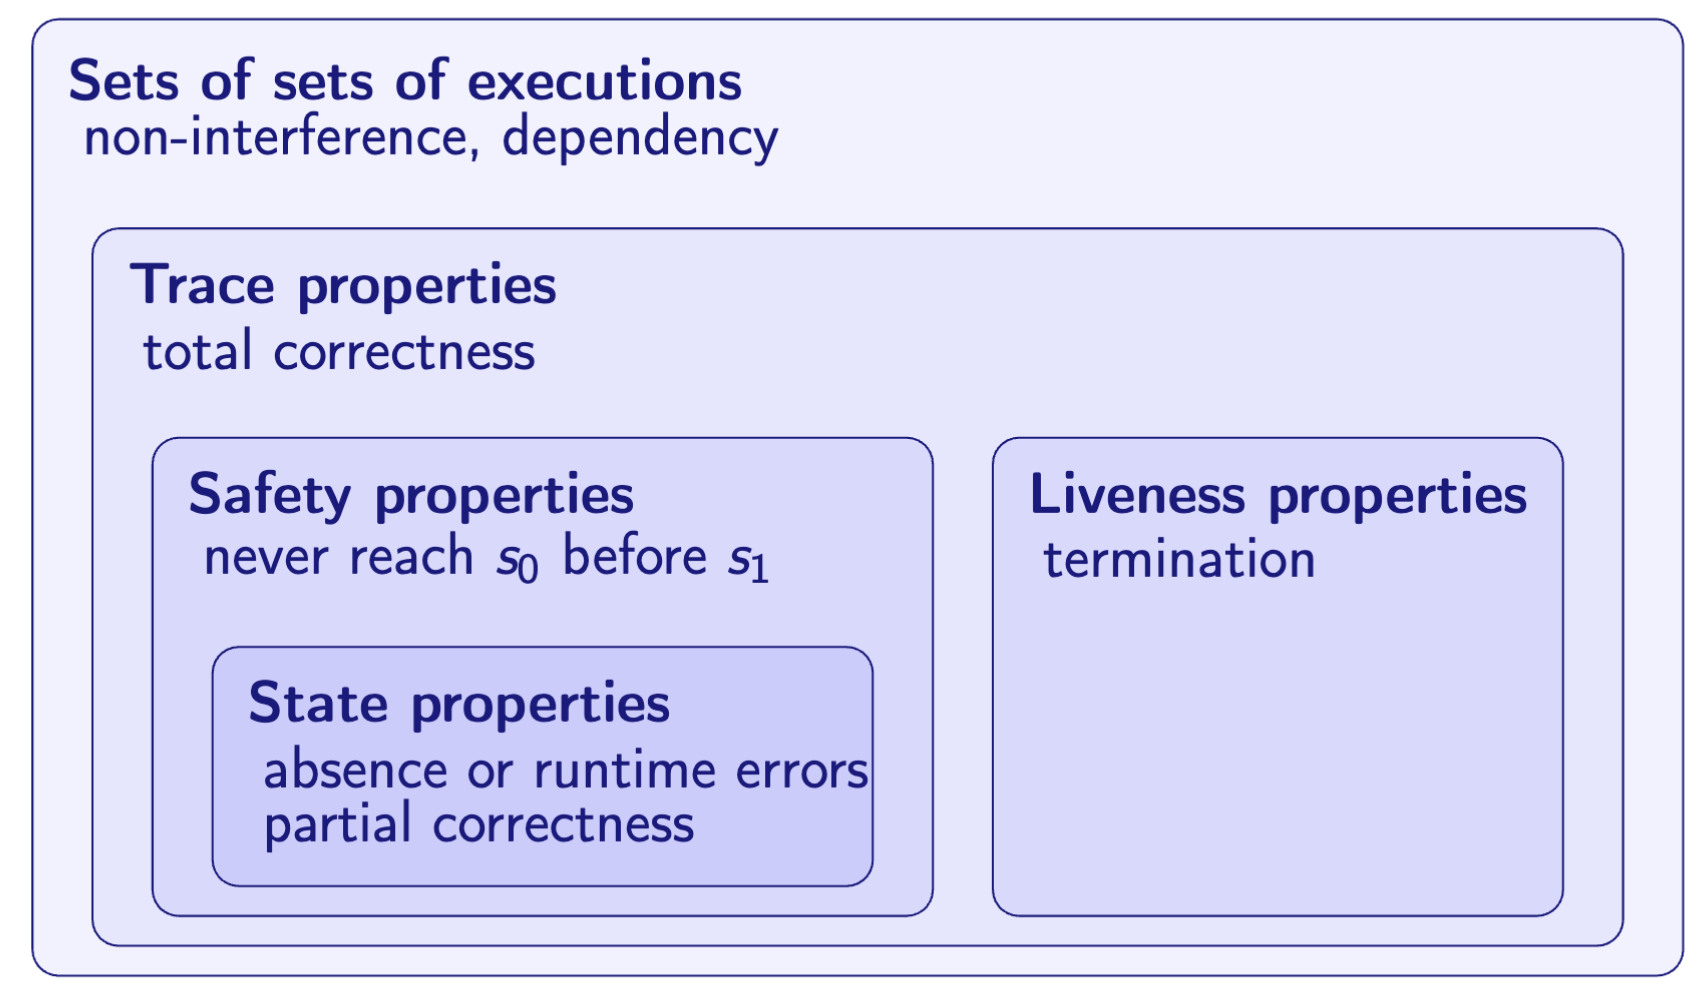
\includegraphics[width=0.7\textwidth]{images/semantic-properties.png}
    \caption{The Zoo of semantic properties}
\end{figure}

Trace properties allow to express a large range of program properties. Safety represents the absence of bad bahaviors, while liveness expresses the existence of good behaviors. Trace properties can be decomposed as conjuctions of safety and liveness properties, with dedicated proof methods. Nevertheless, some interesting properties are not trace properties: we saw that security properties are sets of sets of executions. Finally, the notion of specification languages is usefull to describe program properties.

\section{Denotational semantics}
The first chapters of this class focused on \emph{operational semantics}, through state and trace properties. Such semantics are defined as small execution steps, over low-level internal configurations, with transitions chianed to define maximal traces.

In this chapter, we will delve into denotational semantics. We will study direct function from programs to mathematical objects (denotations), defined by induction on the program syntax (compositional), ignoring intermediate steps and execution details. This is a higher-level, more abstract and modular approach, trying to decouple a program meaning from its execution, and focused on the mathematical structures that represent programs.

Consider the following two programs:
\begin{figure}[H]
    \centering
    \begin{minipage}{0.49\textwidth}
        \centering
        \begin{minted}{c}
int swapped;
do {
    swapped = 0;
    for (int i=1; i<n; i++) {
        if (a[i-1]>a[i]) {
            swap(&a[i-1], &a[i]);
            swapped = 1;
        }
    }
} while (swapped);
        \end{minted}
    \end{minipage}
    \begin{minipage}{.49\textwidth}
        \begin{minted}{ocaml}
let rec sort = function
| [] -> []
| a::rest ->
    let lo, hi = List.partition 
        (fun y -> y < x) rest
    in
    (sort lo) @ [x] @ (sort hi)
        \end{minted}
    \end{minipage}
    \caption{Bubble sort in \texttt{C} (left) and quicksort in \texttt{OCaml} (right)}
\end{figure}
These programs use different languages, algorithms, programming principles and data types; nevertheless, can we give them the same semantics?

We will study two denotation worlds:
\begin{itemize}
    \item Imperative programs, which mutate a memory state. The natural denotation of such a program is an input/output function, over a domain $\mathcal{D} \simeq \textnormal{memory} \rightarrow \textnormal{memory}$.
    \item Functional programs, returning a value without any side effect. One can model a program of type \texttt{a -> b} as a function $\mathcal{D}_a \rightarrow \mathcal{D}_b$.
\end{itemize}

\subsection{Deterministic imperative programs}

\begin{figure}[H]
    \centering
    \setlength\tabcolsep{4pt}
    \begin{grammar}
        \firstrule{\textnormal{expr}}{X}
        \grule{c}
        \grule{\textnormal{expr}}
        \grule{\textnormal{expr} \,\lozenge\, \textnormal{expr}}
    \end{grammar}
    \caption{IMP expressions}
\end{figure}
   

\subsection{Non-determinism}

\subsection{Link between operational and denotational semantics}

\subsection{Higher-order programs}

\subsection{Recursive domain equations}

\newpage
\section{Complement: SAT and Satisfiability Modulo Theories (SMT)}
Since 2000, SAT solvers have become extremely performant. SMT is the extension of SAT with clauses instead of simply variables.
\subsection{Modern SAT solvers}
\subsubsection{The SAT problem}
Given a boolean formula without quantifiers, e.g.
\begin{equation*}
    (p\lor q\lor \lnot r)\land(r\lor \lnot p)
\end{equation*}
we try to find if this formula is satisfiable. Techniques to do so include truth tables, resolution-based procedures, backtracking-based procedure. Since the 80s, there's been a focus on variable selection heuristics, associated with search-pruning techniques (non-chronological backtracking, learning clauses): these are the CDCL algorithms (Conflicts-Driven Clause Learning). New techniques such as indexing and scoring have since emerged.

\subsubsection{Resolution}
Resolution uses a proof-finder procedure, which tries to reduce the equation.

The state of the procedure is represented by a variable $F$, to which we can apply some rules (Resolve, Empty, Tauto, Subsume, Fail). This allows to construct a proof tree.

\subsubsection{DPLL}
DPLL is a model-finder procedure that builds incrementally a model $M$ for a CNF formula $F$ by
\begin{itemize}
    \item deducing the truth value of a literal $l$ from $M$ and $F$ by Boolean Constraint Propagations (BCP):
    \begin{center}
        If $C\lor l\in F$ and $M\vDash \lnot C$ then $l$ must be true
    \end{center}
    \item guessing the truth value of an unassigned literal:
    \begin{center}
        If $M\cup\{l\}$ leads to a model for which $F$ is unsatisfiable\\ then \emph{backtrack} and try $M\cup\{\lnot l\}$
    \end{center}
\end{itemize}

Similarly, DPLL is a set of rules (Success, Unit, Decide, Backtrack, Fail).

\subsubsection{Clause conflict, backjump}
DPLL remains slow: instead of backtracking, we would prefer to \emph{backjump} multiple steps before, to the node where the conflit has indeed been decided. Conflicts are reflected by backjump clauses. Given a backjump clause $C\lor l$, backjumping can undo several decisions at once: it goes back to the assignment $M$ where $M \vDash \lnot C$.

\subsubsection{CDCL algorithm}
Conflict-Driven Clause Learning SAT solvers (CDCL) add backjump clauses to $M$ as learned clauses (or lemmas) to prevent future similar conflicts. 

Lemmas can also be removed from $M$.

The algorithm now has two modes: search and resolution. 

\subsubsection{Heuristics, Two-watched literals}
The Variable State Independent Decaying Sum (VSIDS) heuristic associates a score to each literal in order to select the literal with the hightest score when Decide is used.

CDCL performances are tightly related to their learning clause management. Keeping too many clauses decrease the BCP efficency, but cleaning out too many clauses break the overall learning benefit.

Quality measures for learning clauses are based on scores associated with learned clauses. 

BCP represents 80\% of SAT-solver runtime. The two watched literals technique assigns two non-false watched literals per clause. Only if one of the two watched literal becomes false, the clause is inspected. If the other watched literal is assigned to true, the do nothing. Otherwise, try to find another (unassigned) watched literal. If no such literal exists, then apply Backjump. If the only possible literal is the oother watched literal of the clause, then apply Unit.

Its main advantages are that clauses are inspected only when watched literal are assigned, and that no updating is required when backjumping.

\subsection{Satisfiability Modulo Theories (SMT)}
\subsubsection{Introduction}
The fundamental goal of research in SAT was to be able to solve first-order logic.

The SMT problem asks to decide of the satisfiability of logical formulae with some specific theory symbols. 

In theory, SMT solvers can take as an input any first order logic formula. In pratcice, most SMT solvers only take as input boolean formulas with only one theory (e.g. linear arithmetic over the integers).

\begin{example}
    \begin{equation*}
        f(f(f(x))) = x \land f(f(f(f(f(x))))) = x \land f(x) \neq x
    \end{equation*}

    \begin{equation*}
        x+y = 19 \land x-y=7 \land x\neq 13
    \end{equation*}
\end{example}

Let $F$ be the following formula using arithmetic symbols:
\begin{equation*}
    x+y\geq 0 \land (x=z \implies y+z=-1) \land z > 3t
\end{equation*}
We want to know whether $F$ is satisfiable.
We use the following algorithm:
\begin{figure}[!ht]
    \centering
    \begin{minipage}{0.77\textwidth}
    \begin{enumerate}
        \item Convertion in CNF
        \item Replace arithmetical constraints with boolean variables
        \item Call a SAT solver: a model $M$ is returned if the formula is satisfiable
        \item Convert $M$ to the original theory
        \item Check whether $M$ is coherent with the theory
        \item If not, add $\lnot M$ to $F$ and start over
    \end{enumerate}
    \end{minipage}
    \caption{Simple SMT procedure using a SAT solver}
\end{figure}

SMT encounters multiple difficulties:
\begin{itemize}
    \item The size of formulas (up to multiple Go)
    \item The complexity of boolean structures (e.g. when the formulas encode logical circuits of microprocessors)
    \item The combination of Theories
    \item The efficiency of decision procedures
    \item Theories over mathematical objects more and more complex
    \item The handling of quantifiers
\end{itemize}

\subsubsection{Small proof engines}

\subsubsection{SAT and decision procedures}

\subsubsection{Combination of decision procedures}

\end{document}